\section{Annexes}

\subsection{Planning Actualisé Avant/Après}

Pour notre projet, nous avons opté pour une organisation méthodique en utilisant un tableau Kanban et une répartition des tâches sur GitHub, plutôt que de suivre un planning formel. Le tableau Kanban nous a permis de structurer le travail en plusieurs colonnes : "À faire", "En cours", "À valider" et "Terminé", offrant ainsi une vue d'ensemble claire de l'état d'avancement du projet et facilitant la coordination. Sur GitHub, chaque tâche était associée à une issue, assignée à des membres spécifiques de l'équipe, ce qui a permis un suivi précis des responsabilités et de l'avancement. Cette méthode de travail nous a permis de prioriser les tâches critiques, de tenir des réunions régulières pour synchroniser nos efforts et de rester flexibles face aux imprévus, assurant ainsi une gestion efficace et adaptative du projet, même sans planning détaillé.

\subsection{Liste des Bugs Connus}

\begin{itemize}[noitemsep]
    \item Overflow sur le login
    \item Impossible de lancer la caméra sur Linux ou Chrome
    \item Si un product n'a pas le même id que son docId, il ne peut pas être supprimé
\end{itemize}

\subsection{Dépendances}

\begin{table}[h!]
    \centering
    \begin{tabular}{|m{0.35\textwidth}|m{0.45\textwidth}|}
        \hline
        \textbf{Package}                 & \textbf{Version} \\ \hline
        flutter                          & sdk: flutter     \\ \hline
        injectable                       & \texttt{>2.4.0}  \\ \hline
        flutter\_localizations           & sdk: flutter     \\ \hline
        cupertino\_icons                 & \texttt{>1.0.6}  \\ \hline
        flutter\_clean\_architecture     & \texttt{>5.0.4}  \\ \hline
        firebase\_core                   & \texttt{>2.25.5} \\ \hline
        flutter\_svg                     & \texttt{>2.0.4}  \\ \hline
        syncfusion\_flutter\_charts      & \texttt{>21.2.4} \\ \hline
        shared\_preferences              & \texttt{>2.2.2}  \\ \hline
        jwt\_decoder                     & \texttt{>2.0.1}  \\ \hline
        flutter\_dotenv                  & \texttt{>5.1.0}  \\ \hline
        flutter\_launcher\_icons         & \texttt{>0.13.1} \\ \hline
        flutter\_i18n                    & \texttt{>0.35.1} \\ \hline
        get\_it                          & \texttt{>7.1.3}  \\ \hline
        firebase\_auth                   & \texttt{>4.19.2} \\ \hline
        cloud\_firestore                 & \texttt{>4.17.3} \\ \hline
        provider                         & \texttt{>6.1.2}  \\ \hline
        bloc                             & \texttt{>8.1.2}  \\ \hline
        flutter\_bloc                    & \texttt{>8.1.3}  \\ \hline
        path\_provider                   & \texttt{>2.0.2}  \\ \hline
        auto\_size\_text                 & \texttt{>3.0.0}  \\ \hline
        freezed\_annotation              & \texttt{>2.2.0}  \\ \hline
        camera                           & \texttt{>0.11.0} \\ \hline
        google\_mlkit\_barcode\_scanning & \texttt{>0.12.0} \\ \hline
        http                             & \texttt{>1.2.1}  \\ \hline
        intl                             & \texttt{>0.19.0} \\ \hline
        json\_annotation                 & \texttt{>4.9.0}  \\ \hline
        uuid                             & \texttt{>4.4.0}  \\ \hline
        phone\_number\_controller        & \texttt{>1.0.4}  \\ \hline
    \end{tabular}
    \caption{Dépendances du projet}
    \label{table:dependencies}
\end{table}

\begin{table}[h!]
    \centering
    \begin{tabular}{|m{0.35\textwidth}|m{0.45\textwidth}|}
        \hline
        \textbf{Package}      & \textbf{Version} \\ \hline
        injectable\_generator & \texttt{>2.1.5}  \\ \hline
        build\_runner         & \texttt{>2.0.5}  \\ \hline
        json\_serializable    & \texttt{>6.1.4}  \\ \hline
        freezed               & \texttt{>2.4.7}  \\ \hline
        flutter\_test         & sdk: flutter     \\ \hline
        flutter\_lints        & \texttt{>4.0.0}  \\ \hline
    \end{tabular}
    \caption{Dépendances de développement du projet}
    \label{table:dev-dependencies}
\end{table}


\subsection{Aides Extérieures}

\begin{itemize}[noitemsep]
    \item Documentation officielle de Flutter : \cite{flutterDocs}
    \item Documentation officielle de Firebase: \cite{firebaseDocs}
    \item Documentation de FlutterFire pour l'intégration de Firebase: \cite{flutterFireDocs}
    \item Clean Architecture: \cite{cleanArchitecture}
    \item Figma pour la conception de l'interface utilisateur: \cite{figma}
    \item Design Pattern du Bloc: \cite{blocPattern}
    \item Site de la Migros: \cite{migros}
    \item Site de la Coop: \cite{coop}
    \item Site de Denner: \cite{denner}
    \item Architecture : \cite{googleCloudArchitecture}
    \item Projet existant : un membre du groupe travail sur un projet d'application mobile et le style visuel de l'application a été inspiré de ce projet (couleurs, design, etc.) \url{https://datamama.ch/}
\end{itemize}


\subsection{Wireframe}
\label{doc:wireframe}

\begin{figure}[H]
    \centering
    \includegraphics[width=0.8\textwidth]{images/wireframe.png}
    \caption{Wireframe de l'application}
    \label{doc:wireframe}
\end{figure}

\subsection{Cahier des charges original}

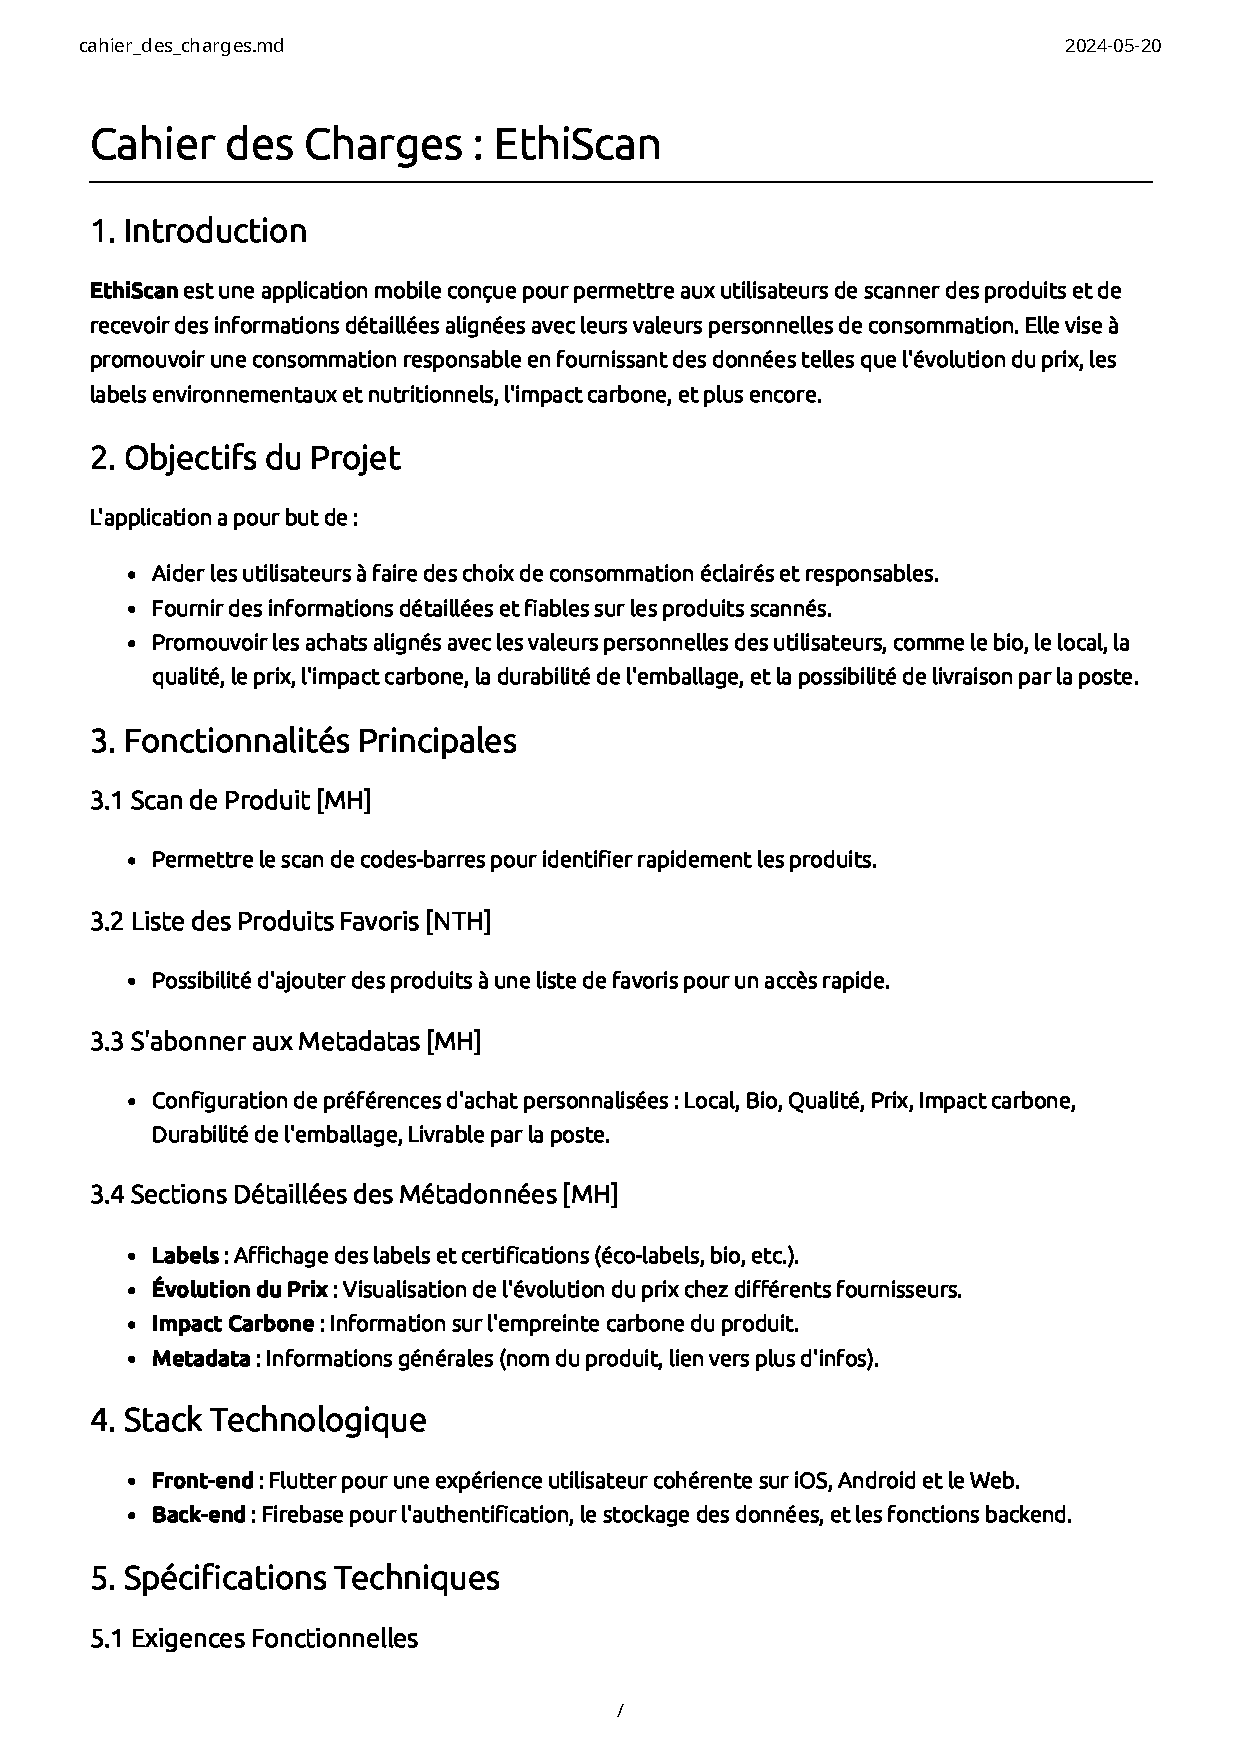
\includepdf[pages=-]{images/cahier_des_charges.pdf}